\documentclass[12pt, a4paper]{article}
\usepackage[utf8]{inputenc}
\usepackage{indentfirst} %indentace prvního odstavce
\usepackage{mathtools}
\usepackage{amsfonts}
\usepackage{amsmath}
\usepackage{amssymb}
\usepackage{graphicx}
\usepackage[czech]{babel}
\DeclarePairedDelimiter{\ceil}{\lceil}{\rceil}

\begin{document}

\section{}
Označme si vybraný počet součástek vektorem $n=(n_{k_1},n_{k_2},n_{t_1},n_{t_2})^T$, kde $n_{k_1}$ odpovídá počtu normálních kondenzátorů, $n_{k_2}$ kvalitních kondenzátorů, $n_{t_1}$ normálních tranzistorů a $n_{t_2}$ kvalitních tranzistorů. Ze zadání víme, že součástka by měla vydržet cca 2.5 roku. Tudíž můžeme shora odhadnout maximální počet každé součastky, protože usoudíme, že součástka by neměla mít větší životnost než 3 roky. Obvod samotný vydrží 1 rok, takže po součástkách chceme dohromady maximálně 2 roky (24 měsíců).

Označme $A = (0.2,0.83,0.85,1.3)$ matici (vektor) \uv{životnosti} a $B = (0.1,1,0.35,0.5)$ matici (vektor) ceny. Jelikož přidaná životnost v měsích součástky sestavené dle vektoru $n$ se spočítá $A \cdot n$ a cena $B \cdot n$.

Maximální počet pro každou součástku je postupně dle značení výše $m_{k_1}=\ceil{\frac{24}{0.2}}=120, \ m_{k_2}=\ceil{\frac{24}{0.83}}=29, \ m_{t_1}=\ceil{\frac{24}{0.85}}=29,\ m_{t_2}=\ceil{\frac{24}{1.3}}=19$. Spočteme si teda všechny možné $n$ tž. $A \cdot n \leq 24$. Takových $n$ existuje 97268.

Chceme minimalizovat hodnotu $(A \cdot n - 18)^2$, 18 značí 1,5 roku, což chceme v optimálním případě, protože součástka přidá 1.5 roku k 1 roku a tedy ve výsledku bude mít $\text{kazítko}^{TM}$ životnost 2,5 roku. Dále samozřejmě chceme minimalizovat cenu což odpovídá hodnotě $(B \cdot n)^2$.

Označme si $\mu$ parametr, který bude značit co ve výsledků více preferujeme (výšší cenu nebo lepší životnost). Pro nějaké $\mu$, chceme tedy minimalizovat hodnotu $(A \cdot n - 18)^2 + \mu \cdot (B \cdot n)^2$ přes všechna možná $n$. Čím větší $\mu$, tak to značí, že dáváme větší důraz na cenu a zanedbáváme životnost. Zde jsou optimální hodnoty pro několik vybraných $\mu$:

\begin{center}
\begin{tabular}{ |c|c|c|c|c|c|c| } 
\hline
$\mu$ & $n_{k_1}$ & $n_{k_2}$ & $n_{t_1}$ & $n_{t_2}$ & \textbf{životnost [měsíce]} & \textbf{cena [Kč]} \\
\hline
0.1 & 0 & 0 & 1 & 13 & 29.75 & 6.85\\
0.2 & 0 & 0 & 1 & 13 & 29.75 & 6.85\\
0.3 & 1 & 0 & 0 & 13 & 29.1 & 6.6\\
0.6 & 0 & 0 & 0 & 13 & 28.9 & 6.5\\
0.7 & 0 & 0 & 1 & 12 & 28.45 & 6.35\\
0.8 & 0 & 0 & 0 & 12 & 27.6 & 6\\
1 & 0 & 0 & 0 & 12 & 27.6 & 6\\
2 & 0 & 0 & 0 & 11 & 26.3 & 5.5\\
4 & 0 & 0 & 0 & 9 & 23.7 & 4.5\\
\hline
\end{tabular}
\end{center}

Doporučujeme zvolit hodnoty pro $\mu=1$, jelikož odchylka předpokládané životnosti 2,5 roku (30 měsíců) je 2,4 měsíce, ale cena je hezkých 6,00,- Kč. Tato hodnota je také vhodná v tom, že potřebujeme pouze součástky jednoho typu (kvalitní tranzistory). Pro jedno $\text{kazítko}^{TM}$ tedy potřebujeme 12 kvalitních tranzistorů.

Zde je zobrazen vývoj pro $\mu$ od 0.1 do 5 (kroky po 0.1). Červený graf značí životnost v měsících a zelený cenu v Kč.
\begin{figure}[h]
\centering
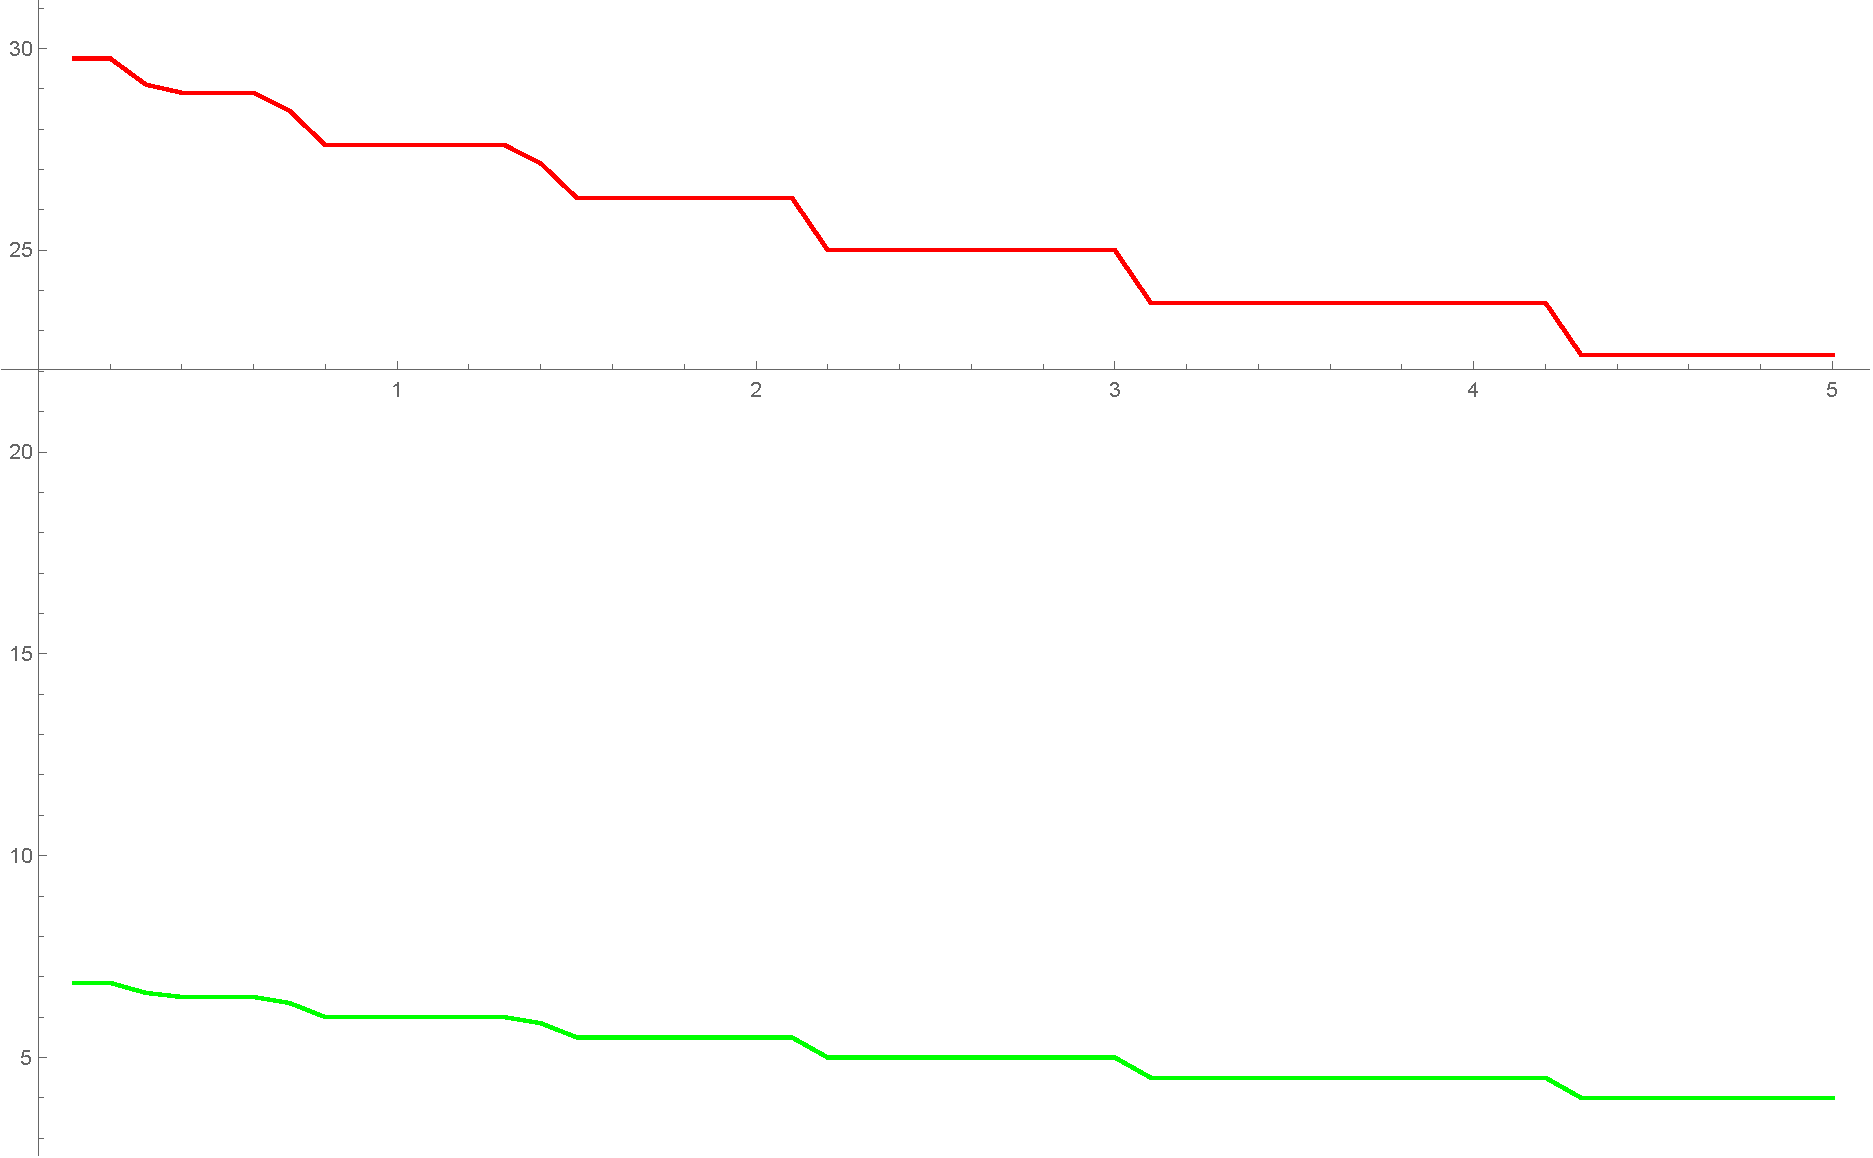
\includegraphics[width=0.8\textwidth]{graf.pdf}
\end{figure}

\section{}
Označme $y(n)$ popularitu politiky v $n$-tém týdnu a $x(n)$ popularitu toaletního papíru. Hledáme model typu Moving Average, který z dat o popularitě toaletního papíru předpoví popularitu politiky. Pro dané $m \in \mathbb{N}$ hledáme váhy $w_1,\dots, w_m \in \mathbb{R}$ tž. platí $y(n)=\sum^{m}_{i=1} w_i \cdot x(n-i)$. Trénovacích dat (týdnů) máme 47. Máme tedy soustavu rovnic:
\[
\begin{pmatrix}
y(m+1)\\
y(m+2)\\
\vdots\\
y(47)
\end{pmatrix}
= 
\begin{pmatrix}
x(m) & x(m-1) & \dots & x(1)\\
x(m+1) & x(m) & \dots & x(2)\\
\vdots & \ddots & \ddots & \vdots\\
x(46) & x(45) & \dots & x(47-m)
\end{pmatrix}
\cdot
\begin{pmatrix}
w_1 \\
w_2 \\
\vdots\\
w_m
\end{pmatrix}
\]

Pomocí metody nejmenších čtverců spočteme $w_1,\dots,w_m$ pro dané $m$. Potřebujeme vybrat ideální $m$, aby tyto parametry nebyly přetrénované ale také dobře předpovídaly. 

Chybu budeme měřit $e_{all} = ||y - \hat{y}||$, kde \\$y = (y(m+1), \dots, y(47), y(48),\dots,y(52))$ kde $y(48),\dots,y(52)$ jsou již testovací data a $\hat{y} = (\hat{y}(m+1),\dots,\hat{y}(52))$ kde $\hat{y}(k)=\sum^{m}_{i=1} w_i \cdot x(k-i)$ neboli data spočítaná z našeho modelu. Dále si změříme chybu $e_{test}=||y_{test}-\hat{y}_{test}||$, kde $y_{test}$ a $\hat{y}_{test}$ jsou jako $y,\hat{y}$ ale pouze s testovacími daty. Máme tedy celkovou chybu modelu a chybu modelu na testovacích datech. 

Zde je graf pro $e_{all}$ (modrá) a $e_{test}$ (červená) pro $m \in \{2,\dots,21\}$ (pokud $m>21$ tak jsou data v podstatě nic neříkající):
\begin{figure}[h]
\centering
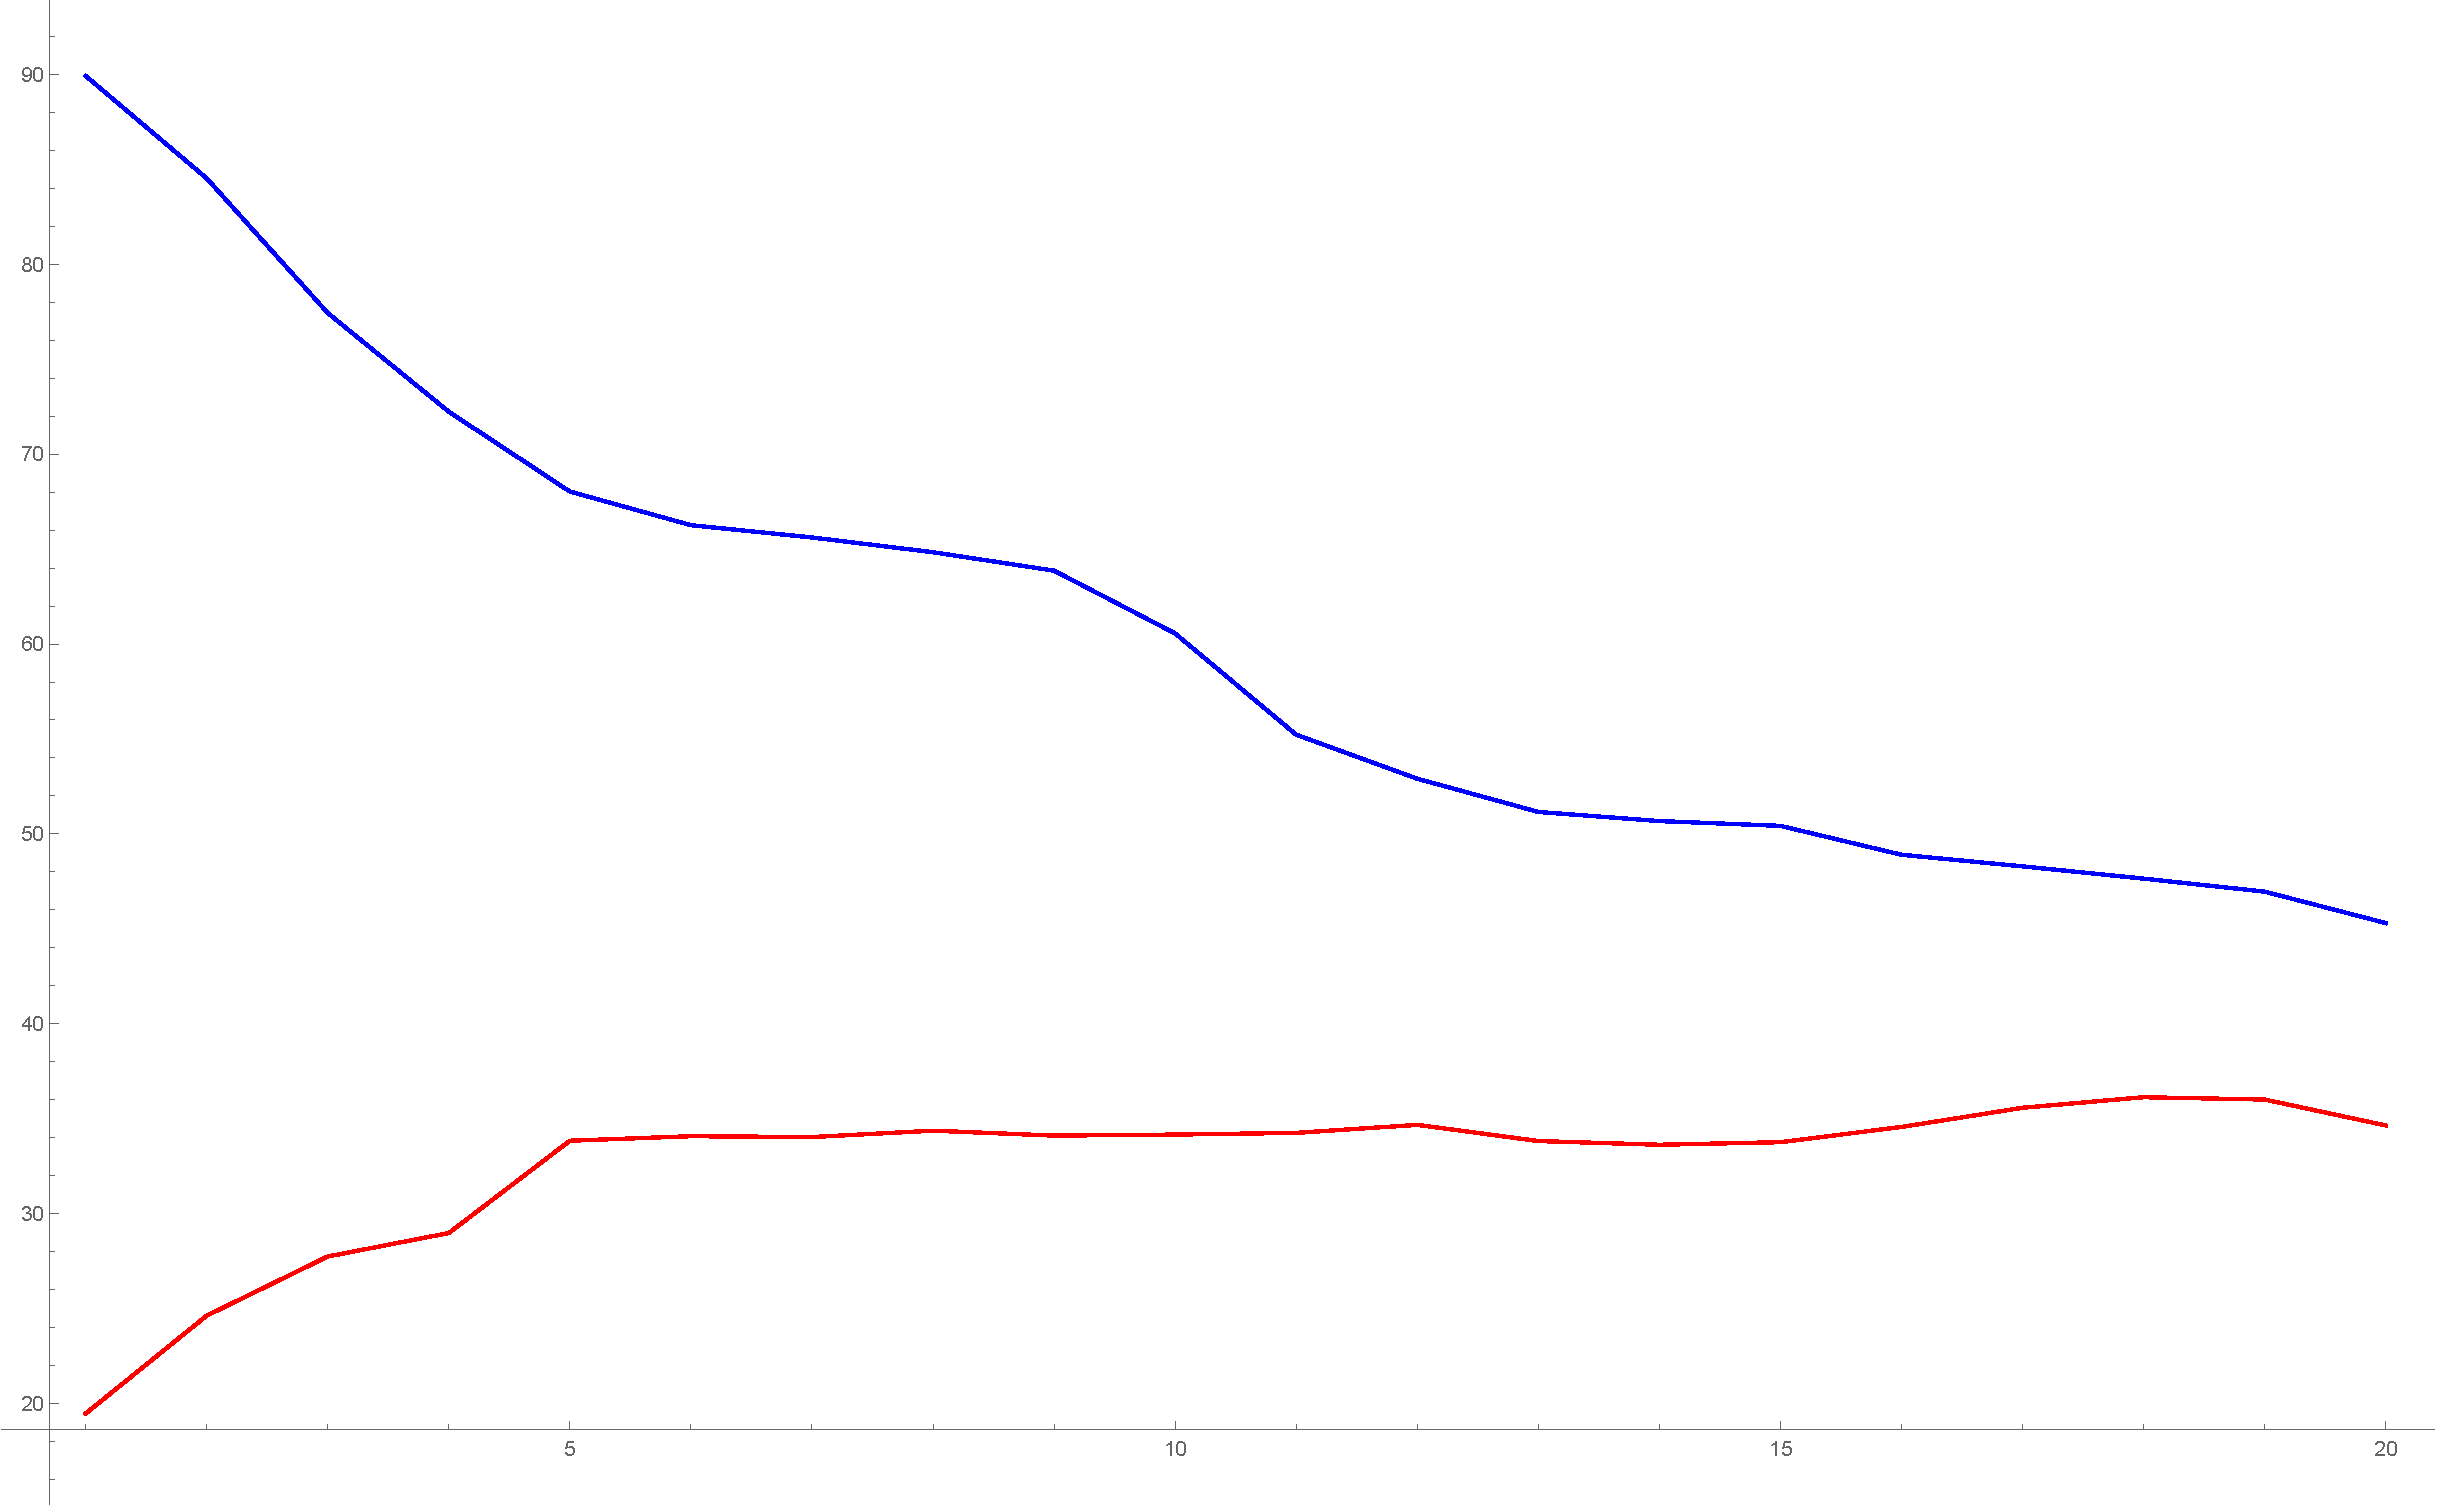
\includegraphics[width=0.8\textwidth]{graf_2.pdf}
\end{figure}

Vidíme že celková chyba stále klesá, jelikož čím dál více přetrénováváme váhy. Vidíme, že model nejlépe funguje pro testovací data pro $m=2$, tedy pouze závilost na 2 předchozích dnech. Zvolme tedy pouze 2 váhy $w_1 = 1.47928, w_2=1.80795$. Zde je graf $y$ (modrá) a $\hat{y}$  (předpověď) pro tyto váhy:
\begin{figure}[h]
\centering
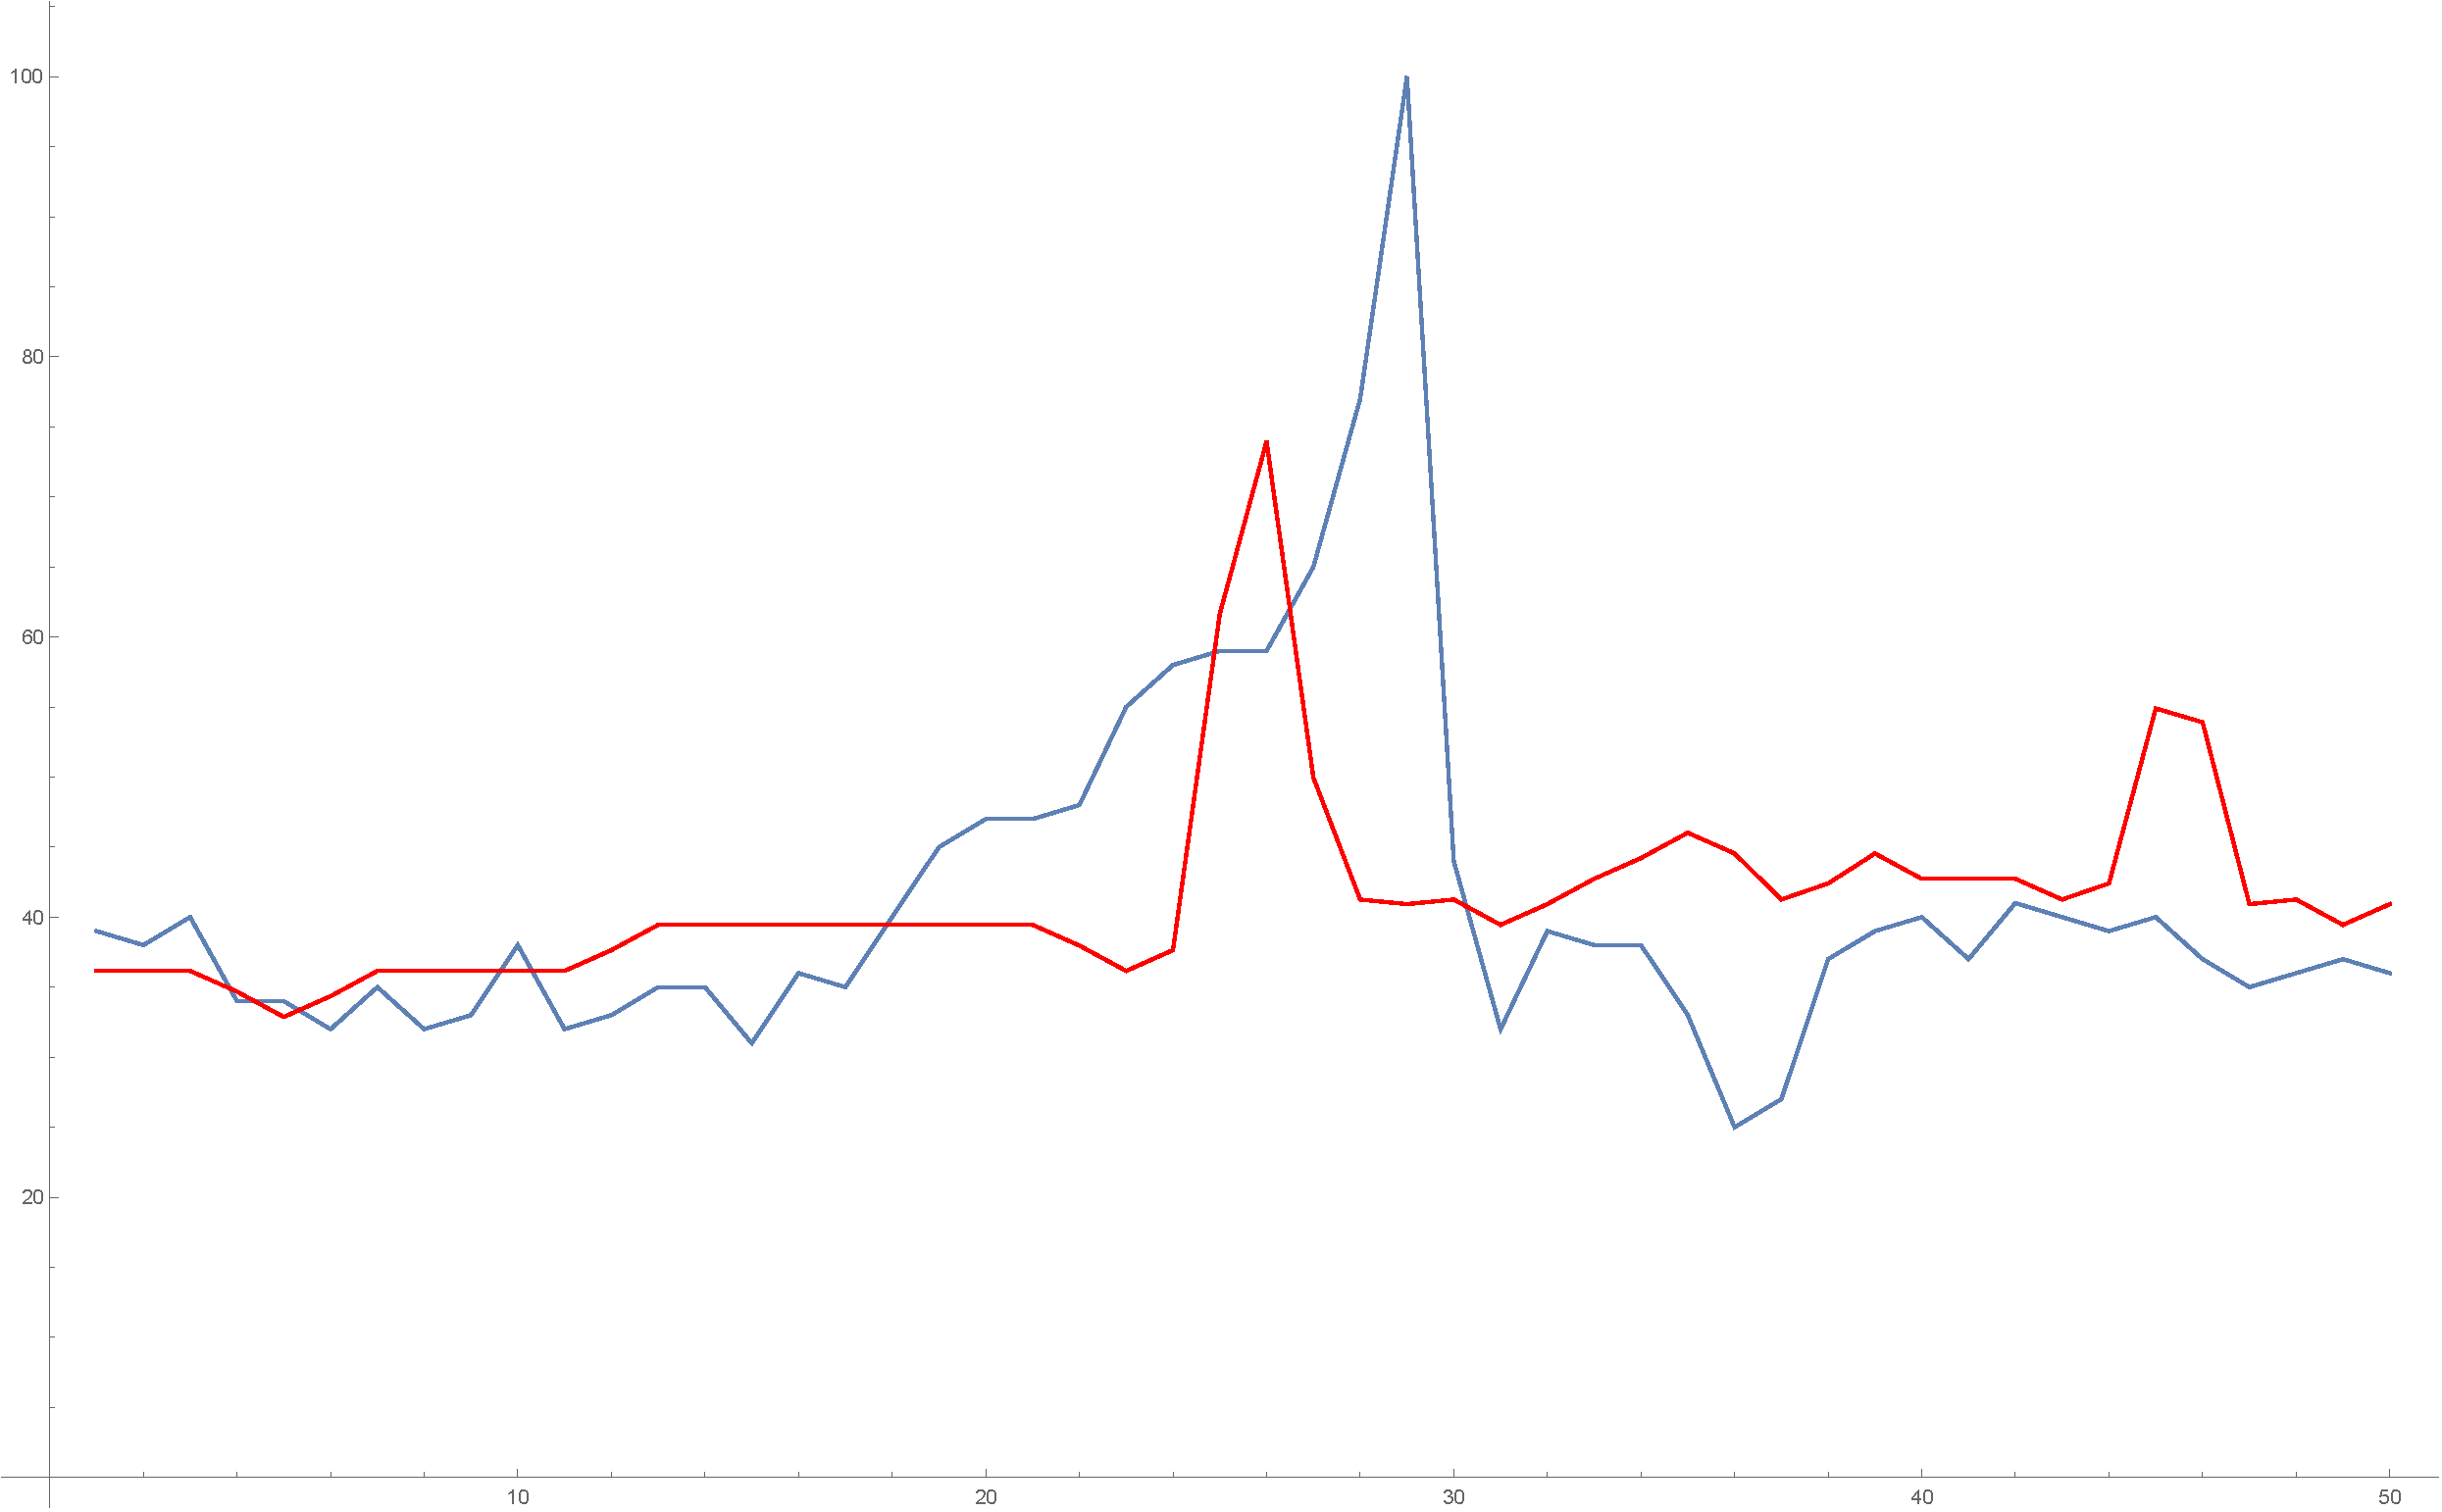
\includegraphics[width=0.8\textwidth]{graf_2_1.pdf}
\end{figure}

\textit{Tématem dnešní politologické rubriky jsou zajímavé korelace. Korelace je matematický termín, který označuje míru závislosti nějaký 2 věcí sobě. Jelikož jsme si všichni prošli Školou života, tak víme, že korelace implikuje kauzalitu. Korelaci, na kterou se dnes podíváme, bude popularita termínů \uv{toaletní papír} a \uv{politika}. Potřebujeme si nějak vysvětlit, proč to tak je. Existuje model, který to předpovídá, takže to musí být pravda. }

\textit{V dnešní době se na internetu nenakupují pouze věci jako elektronika apod., ale i věci co si kupujeme každodenně. Jednou z těch věcí je samozřejmě toaletní papír. Příčina této závislosti je snad nyní zřejmá stejně jako většina věcí, co předpokládají za zřejmé vyučující na jedné nejmenované vysoké škole.}

\textit{Po nakoupení toaletního papíru se český občan již nemusí bát vyhledávat detaily o české politické situaci. Zaskočí-li ho něco, tak se nemusí obávat nedostatku toaletního papíru doma na záchodě. Tohoto fenoménu si nedávno všimnuli provozovatelé podniků, ve kterých se často řeší politická situace. Takovými podniky jsou hlavně hospody a kavárny. Provozovatelé si vytipují do budoucna dny spojené s politikou, a poté nakoupí dostatek toaletního papíru, aby ho byl dostatek, jelikož znají své štamgasty.}

\textit{Nejznámějším dohledatelným případem této „nedostatek toaletního papíru kvůli politické situaci“ krize byla tzv. Velká toaletní krize v Pražské kavárně na konci ledna 2018. Na konci ledna 2018 se konalo druhé kolo volby prezidenta České republiky. Český lid vybíral mezi Milošem Zemanem a Jiřím Drahošem. Je známo, že Pražská kavárna a její pravidelní zákazníci, nemají v oblibě Miloše Zemana. Miloš Zeman také několikrát dal najevo, prostřednictvím svého mluvčího, který mu je věrnější, než byl pes Hachikō svému páníčkovi, že lidi, co navštěvují Pražskou kavárnu (tzv. „lepšolidi“), také nemá rád. Když byl tedy Miloš Zeman zvolen prezidentem, tak za pár minut nebyla v Pražské kavárně jediná role toaletního papíru (popravdě zbyla jedna role jednovrstvého toaletního papíru, ale ten samozřejmě nikdo nechce používat).}

\end{document}